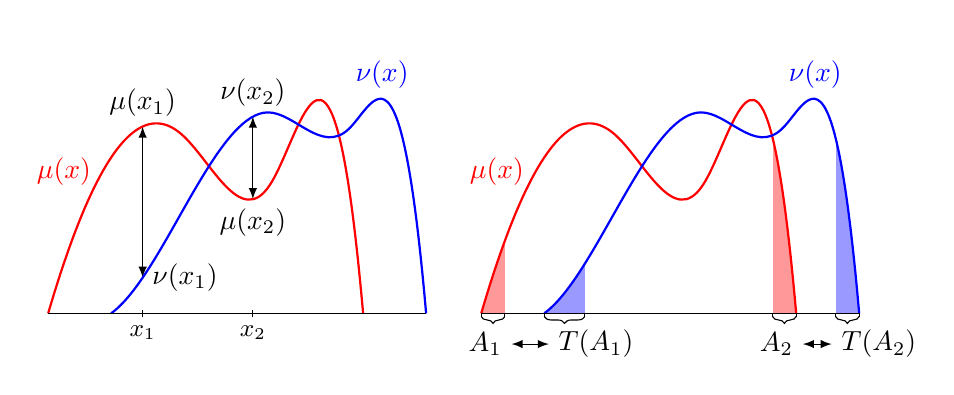
\begin{tikzpicture}[>=latex]
  % Define some colors for consistency
  \def\intensity{0.6}
  \definecolor{lightblue}{rgb}{\intensity, \intensity, 1}
  \definecolor{lightred}{rgb}{1, \intensity, \intensity}
  \def\pathA{(0.000, 0.000) .. controls (0.173, 0.590) and (0.345, 0.976) .. (0.518, 1.131)
   .. controls (0.625, 1.226) and (0.732, 1.233) .. (0.840, 1.143)
   .. controls (1.029, 0.985) and (1.218, 0.528) .. (1.407, 0.814)
   .. controls (1.565, 1.052) and (1.722, 1.807) .. (1.880, 0.975)
   .. controls (1.920, 0.764) and (1.960, 0.450) .. (2.000, 0.000)}
  \def\pathB{(0.000, 0.000) .. controls (0.191, 0.138) and (0.382, 0.541) .. (0.573, 0.857)
   .. controls (0.713, 1.088) and (0.852, 1.272) .. (0.991, 1.276)
   .. controls (1.163, 1.281) and (1.335, 1.008) .. (1.507, 1.169)
   .. controls (1.609, 1.264) and (1.711, 1.512) .. (1.813, 1.238)
   .. controls (1.875, 1.071) and (1.938, 0.709) .. (2.000, 0.000)}
  \def\tickheight{0.02}
  \def\drawscale{2.0}
  \def\xlast{2cm}
  \def\xa{0.6}
  \def\xb{1.3}
  \def\aa{0.15}
  \def\ba{0.258}
  \def\ab{1.85}
  \def\bb{1.850}
  \def\boffset{2.75cm}
  \def\inneroffset{0.4cm}
  \def\arrowoffset{0.8cm}
  \def\bracketoffset{0.35cm}

  % Left Blob (Initial Distribution)
  \begin{scope}[scale=\drawscale,red]
    \draw[<->,black] (\xa, 1.186) node[above]{$\mu(x_1)$} -- (\xa, 0.226) node[right]{$\nu(x_1)$};
    \draw[<->,black] (\xb, 0.725) node[below]{$\mu(x_2)$} -- (\xb, 1.249) node[above]{$\nu(x_2)$};
    \draw[thick] \pathA;
    \node at (0.1cm, 0.9cm) {$\mu(x)$};
    % Right Blob (Transformed Distribution)
    \begin{scope}[xshift=\inneroffset,anchor=south west,color=blue]
      \draw[thick] \pathB node[pos=-0.5,above]{$\nu(x)$};
    \end{scope}

    % Draw Axes
    \begin{scope}[font=\small]
    \draw[black] (0,0) -- (\xlast+\inneroffset,0);
    \draw[black] (\xa,-\tickheight) -- (\xa,\tickheight)
      node[pos=0,anchor=north]{$x_1$} ;
    \draw[black] (\xb,-\tickheight) -- (\xb,\tickheight)
      node[pos=0,anchor=north]{$x_2$} ;
    \end{scope}
  \end{scope}

  % Left Blob (Initial Distribution)
  \begin{scope}[scale=\drawscale,xshift=\boffset,red]
    \begin{scope}[lightred]
      \clip \pathA;
      \fill (0, 0.0) rectangle (\aa, 1.5);
      \fill (\ab, 0.0) rectangle (\xlast, 1.5);
    \end{scope}
    \draw[thick] \pathA;
    \node at (0.1cm, 0.9cm) {$\mu(x)$};
    % Right Blob (Transformed Distribution)
    \begin{scope}[xshift=\inneroffset,anchor=south west,color=blue]
      \begin{scope}[lightblue]
        \clip \pathB;
        \fill (0, 0.0) rectangle (\ba, 1.5);
        \fill (\bb, 0.0) rectangle (\xlast, 1.5);
      \end{scope}
      \draw[thick] \pathB node[pos=-0.5,above]{$\nu(x)$};

      \begin{scope}[black]
        \draw (0,0) -- ++(0, -\tickheight) coordinate (b1tickstart);
        \draw (\ba,0) -- ++(0, -\tickheight) coordinate (b1tickend);
        \draw (\bb,0) -- ++(0, -\tickheight) coordinate (b2tickstart);
        \draw (\xlast,0) -- ++(0, -\tickheight) coordinate (b2tickend);
        \draw[decorate,decoration={brace,mirror}] (b1tickstart) -- (b1tickend)
          node[midway,below=\bracketoffset,anchor=center,xshift=0.4cm](b1end) {$T(A_1)$};
        \draw[decorate,decoration={brace,mirror}] (b2tickstart) -- (b2tickend)
          node[midway,below=\bracketoffset,anchor=center,xshift=0.4cm](b2end) {$T(A_2)$};
      \end{scope}
    \end{scope}
    \begin{scope}[black]
      \draw (0,0) -- (\xlast+\inneroffset,0);

      \draw (0,0) -- ++(0, -\tickheight) coordinate (a1tickstart);
      \draw (\aa,0) -- ++(0, -\tickheight) coordinate (a1tickend);
      \draw (\ab,0) -- ++(0, -\tickheight) coordinate (a2tickstart);
      \draw (\xlast,0) -- ++(0, -\tickheight) coordinate (a2tickend);
      \draw[decorate,decoration={brace,mirror}] (a1tickstart) -- (a1tickend)
        node[midway,below=\bracketoffset,anchor=center,xshift=-0.1cm](a1end){$A_1$};
      \draw[decorate,decoration={brace,mirror}] (a2tickstart) -- (a2tickend)
        node[midway,below=\bracketoffset,anchor=center,xshift=-0.1cm](a2end) {$A_2$};
      \draw[<->] (a1end) -- (b1end);
      \draw[<->] (a2end) -- (b2end);
    \end{scope}
  \end{scope}


\end{tikzpicture}
